\documentclass[10pt,twocolumn]{article}
\usepackage[letterpaper,left=.74in,right=.74in,top=.67in,bottom=.67in,columnsep=.24in]{geometry}
\usepackage[T1]{fontenc}
\usepackage{graphicx,booktabs,amsmath,microtype}
\usepackage[hidelinks]{hyperref}
\setlength{\emergencystretch}{1em}
\setlength{\textfloatsep}{12pt plus 2pt minus 2pt}
\setlength{\dbltextfloatsep}{12pt plus 2pt minus 2pt}
\linespread{.97}
\raggedbottom
\setcounter{topnumber}{3}
\setcounter{dbltopnumber}{3}
\renewcommand{\topfraction}{.9}
\renewcommand{\dbltopfraction}{.92}
\renewcommand{\textfraction}{.08}
\title{\bfseries State-Aware Data Minimization for Tool-Using Agents\\
\large Revalidating Reads When Business State Changes}
\author{Anonymous authors}
\date{}
\begin{document}
\maketitle

\begin{abstract}
In a tool-using agent, a field can be needed when a read is prepared and become unnecessary before the tool returns its raw value. Business-state changes can invalidate the reason for the read while task authorization stays fixed. We enforce field necessity at delivery and return value-free recovery feedback on denial. The agent can then replan, reuse applicable checks and committed work, or stop if no authorized route remains. In paired refund and logistics experiments with two hosted models, enforcement reduces stale field deliveries from 144 to zero per model relative to agent-directed reads. Per-policy business completion is 359/360 with Qwen3.8-Flash and 360/360 with Qwen4-Max. The guard recovers after 119 and 120 of 120 blocked reads, respectively. In a 270-run transfer study using independently developed $\tau$-bench retail tools, both a refreshed composable route table and a versioned contract verifier reduce excess field deliveries from 270 to zero, with 90/90 correct outcomes per arm. In a separate strong-baseline comparison with Qwen4-Max, version binding adds 90 read denials and 360 pre-closure tool calls when the route remains valid after an evidence update. A controlled Gaia2 replay shows that moving the check to delivery blocks stale replies with either backend. Narrowing grant dependencies removes three avoidable denials and twelve tool calls in a paired refund study. A compositional rule-change study measures identical authored changes and audit coverage for both backends, with different generated representations.
\end{abstract}

\section{Introduction}
A user asks an agent to prefer a wallet refund and use a bank refund if the wallet is unavailable. The wallet is initially unavailable, so the agent selects the bank route and prepares to read account fields. While that request is pending, the wallet becomes available. The user's authorization stays fixed, yet their stated preference now makes the bank fields unnecessary. The same read can be justified at preparation and unjustified at delivery.

This timing matters because the model can see a raw value as soon as a tool releases it. A later action check can prevent the agent from executing the bank refund, but the account fields are already in model context. Section~\ref{sec:refund-maintenance} separates this failure from task completion using an upstream cancellation and a controlled delivery window. Business completion therefore tells us whether the workflow ended correctly. Measuring the fields actually delivered tells us whether the agent received data it no longer needed. Upfront minimization, as in AirGapAgent~\cite{airgap}, limits what the agent initially sees and provides a path for escalation. We examine the status of an individual read after execution begins, when the agent's earlier evidence can become stale.

Our design checks necessity at the connector, just before the value crosses into model context. The connector checks whether the pending step belongs to a currently admissible plan, whether its prerequisites hold, and which inputs it still needs. A denied read returns a reason and authorized recovery options without releasing new raw values. The agent issues the next tool call. It can refresh state, choose an eligible route, retain valid verification and committed work, or stop safely if no authorized continuation remains.

We compare two ways to enforce that boundary. A refreshed composable route table recomputes necessity from the current state on each read. A contract verifier derives step requirements from tool contracts and also checks the versions bound to a previously issued grant. In the refund example, both can block the bank fields once the wallet becomes available. If an evidence record changes while the bank route remains eligible, the table can release the still-needed fields and the verifier can require a fresh grant. Our evaluations measure this distinction separately from genuine route changes.

\paragraph{Contributions.}
\begin{enumerate}
\item We formulate \emph{necessity at delivery} for step-level agent reads. The formulation connects authorization, route preference, prerequisites, and current evidence, and states the conditions for enforcing necessity at the connector.
\item We implement delivery-time checks with two backends and specify a shared recovery path. Agent tool calls can refresh evidence, preserve completed effects, reuse valid verification, and stop when the original authorization provides no continuation.
\item We quantify field exposure, recovery, and tool costs in matched autonomous experiments across two hosted models and an independently developed retail tool environment. Refreshed route tables achieve the same zero excess releases as the contract verifier in the direct comparisons. The version-only condition identifies cases in which stricter evidence binding adds recovery work while current necessity stays unchanged.
\end{enumerate}

\section{Problem and trust model}
\paragraph{Actors and state.}
A user supplies a goal set $G$, data authorization $U$, and an ordering over acceptable options. The authorized route set is subject to business facts, such as availability, and already completed actions. The model may misread policy, act on stale information, or follow instructions in untrusted tool text. A trusted tool registry and business connector define action contracts and provide authenticated, versioned evidence. We assume that the relevant private output is mediated by the connector. Bypassed tools or compromised state sources are outside this boundary.

\paragraph{Necessity at delivery.}
Let $C$ be the trusted tool contracts and $E_t$ the evidence available at time $t$. A plan is admissible if its actions are authorized, its preconditions have trusted support, and it obeys the configured user preference. When a condition is unknown, the platform can withhold the plan pending evidence if learning that condition could change plan acceptance. Permission to use a value for an authorized task supplies an upper bound on access. Whether that value is needed now depends on the enabled step within an admissible plan.

We distinguish \emph{decision information} from \emph{execution inputs}. A fixed predicate, such as whether a fee is below a user-approved threshold, can inform a plan without delivering the exact fee. The predicate result still conveys information. Conversely, an explicit reporting goal may require exact values, including a quote from a route that the agent ultimately does not execute.

\paragraph{Security objective.}
For a mediated read, the connector releases only the fields missing for the pending step of a plan it currently accepts. This objective is conditional on correct contracts, current trustworthy evidence, and mediated access. It does not characterize downstream use of a legitimate input. We measure visible output separately and make no claim about hidden reasoning or provenance-aware output control.

\section{Delivery-time minimization}
\label{sec:method}

\subsection{Running example and enforcement boundary}
The user asks for one refund, preferring the wallet and authorizing the bank as fallback if the wallet is unavailable. A trusted status response initially marks the wallet unavailable and the bank available. The agent proposes the bank route. Its pending account verification step needs an account reference and an owner reference. Before those references enter model context, the wallet recovers. Both backends deny the old request and give the agent the same safe recovery options. The agent then proposes the wallet route, reads its wallet reference and obtains the required confirmation before executing the refund (Figure~\ref{fig:refund-sequence}).

The agent controls which actions and fields it requests. The connector controls which raw values cross into model context. Above that boundary, both backends expose the same user authorization, route preferences, status queries, approval policy and recovery interface. Below it, the \emph{refreshed route table} composes reusable route recipes and evaluates route, prerequisite and field rules from the current snapshot. The \emph{contract verifier} derives step requirements from tool contracts, binds a read grant to its supporting evidence and revalidates it at delivery. The stores and trusted state interface are shared. Figure~\ref{fig:mechanism} locates each decision and the common release point.

\begin{figure*}[t]
\centering
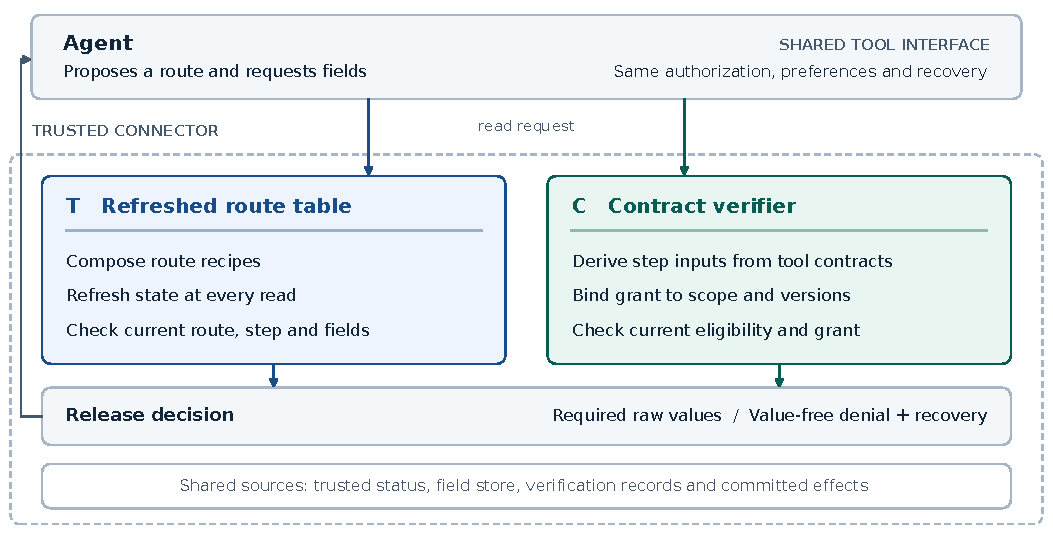
\includegraphics[width=\textwidth]{figures/backend-comparison.pdf}
\caption{Both backends enforce the same delivery boundary. The route table derives permission anew from the current snapshot at every read. The contract verifier additionally checks that the evidence and values bound to an earlier grant still match. Each backend returns permitted values or a value-free denial through the same tool interface.}
\label{fig:mechanism}
\end{figure*}

\subsection{Selecting a plan with incomplete evidence}
A tool step $a$ declares required and produced artifacts, required raw fields $R_a$ and business predicates. A plan joins steps that can achieve the remaining goals from the available artifacts. $\mathcal P_U$ contains only plans whose tools and fields fall within the user's authorization $U$. The route table obtains candidates from configured recipes. The contract backend derives them from artifact production and consumption.

Let $B(p)$ be the required literals for plan $p$. The evidence view $E_t$ contains current known true literals. If neither a literal nor its negation appears, its truth is unknown. Let $\overline{B(p)}$ be the pointwise negation of $B(p)$. The possible and proven sets are
\begin{align}
P_t &= \{p\in\mathcal P_U : E_t\cap\overline{B(p)}=\emptyset\},\label{eq:possible}\\
K_t &= \{p\in P_t : B(p)\subseteq E_t\}.\label{eq:proven}
\end{align}
Let $\rho(p)$ order plans by user preference and, if configured, by disclosure cost as a tie-breaker. Lower is better. With $r_t=\min_{p\in K_t}\rho(p)$ and $\min\emptyset=+\infty$, the unresolved higher-priority set and the admissible plans are
\begin{align}
Q_t &= \{p\in P_t\setminus K_t : \rho(p)<r_t\},\label{eq:unresolved}\\
A_t &=
\begin{cases}
\{p\in K_t:\rho(p)=r_t\}, & Q_t=\emptyset,\\
\emptyset, & Q_t\ne\emptyset .
\end{cases}\label{eq:admissible}
\end{align}
The agent proposes a plan. The backend checks whether it is in $A_t$. If $Q_t$ is nonempty, status evidence for those unresolved plans must be obtained first. For example, confirmed bank availability alone does not establish fallback while wallet availability is unknown. Evidence of wallet unavailability excludes the wallet plan and can make the bank plan admissible.

\subsection{Deciding what to release}
Write $X_t=(E_t,\eta_t,\nu_t,H_t,M_t,L_t)$ for a trusted snapshot. Here $\eta_t$ and $\nu_t$ map predicates and values to versions with fresh identifiers on update, $H_t$ holds verification records, $M_t$ holds fields already delivered at their current version, and $L_t$ is the ledger of committed effects. Let $s$ denote a plan session on resource $r$, with plan $p_s$. For an enabled step $a$ in that session, the missing raw fields are
\begin{equation}
D_t(a)=R_a\setminus M_t.\label{eq:missing}
\end{equation}
An enabled step is pending, has its prerequisites satisfied and respects confirmation requirements applicable at that step. For the two backends we use the following common release predicate. $S$ is the set of fields in the request, after rejecting duplicate field identifiers. Scope checks the resource, session and step.
\begin{align}
\mathrm{Allow}_t(r,s,a,S)={}&
\mathrm{Scope}(r,s,a) \land p_s\in A_t \notag\\
 &{}\land\mathrm{Enabled}_t(s,a)
 \land S=D_t(a).\label{eq:common-guard}
\end{align}
The route table refreshes $X_t$ for each read, resolves the matching route recipe and applies Eq.~\eqref{eq:common-guard} using its field and prerequisite rules. A contract read first obtains a single-use grant
\begin{equation}
g=(r,s,a,D_i(a),\sigma_s,\nu_i|_{D_i(a)}),\label{eq:grant}
\end{equation}
where $i$ is the issue time and $\sigma_s$ holds the predicate versions captured for the accepted session. This includes relevant evidence excluding a preferred alternative. The reference implementation conservatively tracks known predicates across permitted plans. For redemption, in addition to Eq.~\eqref{eq:common-guard}, the request must satisfy
\begin{align}
 &\mathrm{Unused}(g)\land\mathrm{Match}(g,r,s,a,S)\notag\\
 &{}\land\eta_t|_{\mathrm{dom}(\sigma_s)}=\sigma_s
 \land\nu_t|_S=\nu_i|_S .\label{eq:grant-valid}
\end{align}
$\mathrm{Match}$ binds the request to the grant's scope and field set. The current plan check remains necessary because resolving a previously unknown predicate can change $A_t$ without changing an entry recorded in $\sigma_s$. A tracked change can also invalidate the grant while the same plan remains admissible. The refreshed table can allow such a read when the current step and requested fields still satisfy its rules.

\begin{figure*}[t]
\centering
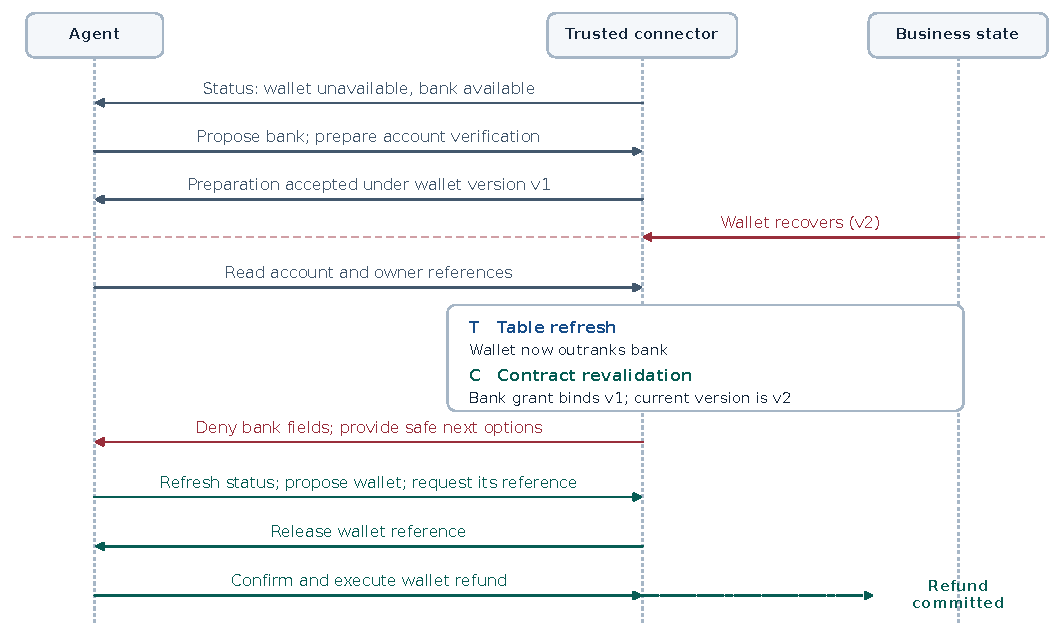
\includegraphics[width=\textwidth]{figures/refund-sequence.pdf}
\caption{Worked refund trace, with the two backend outcomes shown as alternatives for the same request. Wallet availability changes from false to true before delivery. The table excludes the now lower-priority bank route. The contract verifier also sees that its grant binds the previous wallet version. Both return a denial without bank data. The agent proposes and completes the wallet route. Versions are illustrative.}
\label{fig:refund-sequence}
\end{figure*}

\subsection{Safety property}
\textbf{Proposition 1 (necessity at delivery).}
Assume (i) all raw reads in scope pass through the trusted connector, (ii) authorized routes and step-field rules faithfully specify business prerequisites and required fields, and (iii) the authorization check and value release are evaluated against the same current snapshot. If either backend releases any raw fields for a step, the step is enabled on a currently admissible plan and the released fields are exactly its missing required set $D_t(a)$. In contract mode, changing a tracked predicate or bound field version invalidates the old grant.

\emph{Proof.} For every release, Eq.~\eqref{eq:common-guard} requires membership in $A_t$, scope, step eligibility and equality to $D_t(a)$. By (iii), the released values correspond to that same snapshot. A failed conjunct yields a denial with no raw values. The contract verifier also requires both version equalities in Eq.~\eqref{eq:grant-valid}. A changed bound version makes its equality false. In the refund trace, the wallet recovery removes the bank plan from $A_t$ and changes the wallet predicate version in the bank grant. Thus either backend denies the old read.\hfill\rule{.6ex}{.6ex}

The evaluated simulator processes validation and delivery sequentially. A concurrent connector needs an atomic conditional read or an equivalent version-checked transaction before this property applies. The result concerns release of raw values via the connector. It leaves inference from status signals, reuse of already delivered values and disclosure in model output outside the guarantee.

\subsection{Recovery after rejection}
A denial supplies a reason, valid artifacts already available and safe next options within $U$. It carries no newly read raw values. Let $X'$ be the refreshed state and $G$ the original goals. The shared recovery rule filters reusable records and current-value markers and replans against the ledger:
\begin{align}
H' &= \{h\in H : \mathrm{Valid}(h,X',r,U)\},\label{eq:reuse}\\
M' &= \{f\in M : \nu'(f)=\mathrm{SeenVersion}(f)\},\label{eq:seen}\\
G_{\mathrm{left}} &= G\setminus\mathrm{Done}(L).\label{eq:remaining}
\end{align}
Verification reuse requires the same resource and an allowed purpose, plus current relevant versions. Here $M'$ changes what may be treated as current by the connector. It does not erase earlier model context. The ledger stays fixed during replanning. Subsequent successful business operations can extend it. If no authorized continuation exists, the agent stops, or asks for new consent only when the shared approval policy permits it.

In the worked refund trace, the ledger has no committed refund when the bank read fails. The agent selects the wallet and issues new calls, and only the wallet reference is delivered. In a separate reuse case, an earlier identity verification can carry across the route change if Eq.~\eqref{eq:reuse} holds. The scripted adapters implement reuse for supported verification records and business effects.

\begin{table}[t]
\small
\centering
\begin{minipage}{.98\columnwidth}
\hrule\vspace{4pt}
\textbf{Algorithm 1. Select and read}\\[2pt]
\textbf{Select:} derive candidates for remaining goals\\
\quad compute $Q_t$ and $A_t$ (Eqs.~\ref{eq:unresolved}--\ref{eq:admissible})\\
\quad \textbf{if} $Q_t\ne\emptyset$: request status evidence\\
\quad \textbf{if} $A_t=\emptyset$ and $Q_t=\emptyset$: report no route\\
\quad validate the agent's proposed plan against $A_t$\\
\textbf{Prepare (contract):} issue the grant (Eq.~\ref{eq:grant})\\
\textbf{Read:} obtain the delivery snapshot\\
\quad table: resolve the current recipe and check Eq.~\eqref{eq:common-guard}\\
\quad contract: check Eqs.~\eqref{eq:common-guard} and \eqref{eq:grant-valid}\\
\quad \textbf{if} a check fails: deny with safe feedback\\
\quad release permitted values and consume any grant
\vspace{4pt}\hrule
\end{minipage}
\end{table}

\begin{table}[t]
\small
\centering
\begin{minipage}{.98\columnwidth}
\hrule\vspace{4pt}
\textbf{Algorithm 2. Continue after a denied read}\\[2pt]
\textbf{Agent:} refresh status using a permitted tool\\
\quad use the backend's valid records and remaining goals\\
\quad query unresolved evidence if needed\\
\quad \textbf{if} no authorized continuation: stop or seek consent\\
\quad propose a plan and issue fresh calls for its missing inputs\\
\quad confirm as required, then call the business action\\
\textbf{Backend:} check prerequisites and record committed effects
\vspace{4pt}\hrule
\end{minipage}
\end{table}


\section{Evaluation}
\subsection{Autonomous model experiment}
\label{sec:autonomous}
We compare three policies. \textsc{Upfront} returns all task-authorized candidate inputs in its first state inspection. \textsc{Agent only} lets the model request inputs as needed while preserving task-level authorization and common plan and execution checks. A shadow check records when a request would violate step-level necessity. \textsc{State guard} enforces necessity at delivery. The upfront arm isolates an eager-release policy and should be interpreted separately from the dedicated AirGap-style adaptation.

The main experiment consists of 120 parameterized synthetic tasks across refund and logistics, grouped into 60 pairs. Paired members share the user request, profile and rules, with different business state. The suite balances single-route, route-switch and multiple-stage workflows, 40 of each. We run all three policies with each of two hosted model aliases (\texttt{qwen3.8-flash} and \texttt{qwen4-max}), native tool calls and shared task authorization, approval and recovery rules. Each task runs with three seeds, yielding 360 attempts per policy. The archived protocol fixes temperature 0.3, a budget of 40 model responses, a 512-token output cap per response, and two recoveries. We retain incomplete attempts and distinguish HTTP retries from returned model calls.

In route-switch tasks, the simulated condition can change after the first read justification and before field delivery. The event occurred in all 120 attempts in each on-demand arm for both models. In the upfront arm it occurred in 108 of 120 Qwen3.8-Flash attempts and all 120 Qwen4-Max attempts. Some Qwen3.8-Flash workflows used already supplied values and skipped the triggering action. Event exposure in the upfront comparison therefore varies by model. The primary comparison uses the two on-demand arms.

\paragraph{Metrics and uncertainty.}
An independent task ledger determines successful business effects and applicable confirmations. We separately count unique raw field instances (deduplicated within an attempt), fields unused by the resulting valid execution, and fields released despite a stale evidence check. These counts may overlap. We count successful business effects even when the expected final answer fails to arrive, and report final-answer completion separately. We check visible model prose and simulated external text for exact synthetic value matches. The protocol does not observe paraphrases, partial disclosures, or hidden reasoning. Intervals use 5,000 paired cluster bootstrap draws over the 60 state pairs, with both members and all repeats kept together. They describe uncertainty for this constructed suite, rather than a production workload.

\begin{table*}[t]
\centering
\small
\begin{tabular}{@{}lrrrrrrrr@{}}
\toprule
Policy & Business success & Raw fields & Unused & Stale & Tool calls & Model calls & Approvals & Leaks \\
\midrule
Upfront & 359/360 & 1752 & 1049 & 1 & 2775 & 3134 & 139 & 1 \\
Agent only & 359/360 & 850 & 144 & 144 & 3487 & 3840 & 141 & 0 \\
State guard & 359/360 & 707 & 0 & 0 & 3446 & 3806 & 141 & 1 \\
\bottomrule

\end{tabular}
\caption{Autonomous comparison across 360 attempts per policy and model (2,160 total). Field instances are deduplicated within attempts and summed. Leaks counts trajectories with a visible exact-value disclosure. Approvals are simulated. Repeated HTTP transport attempts are excluded from the model calls column.}
\label{tab:autonomous}
\end{table*}

\begin{figure*}[t]
\centering
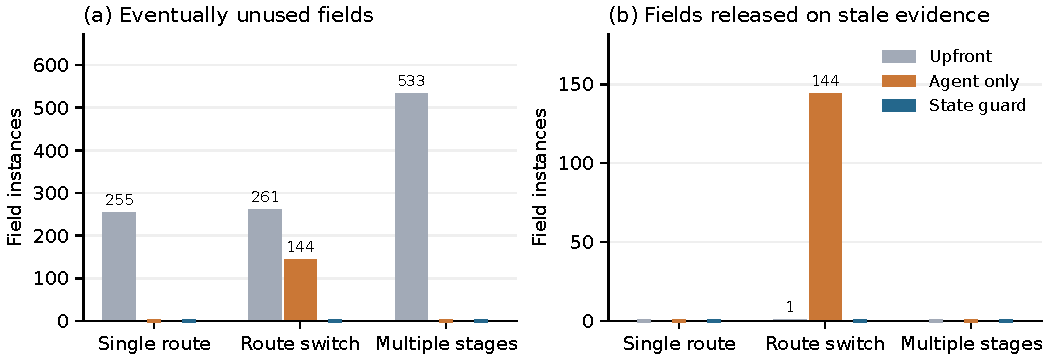
\includegraphics[width=.92\textwidth]{figures/exposure.pdf}
\caption{Qwen3.8-Flash field exposure by workflow family (120 attempts per policy per family). Zero counts appear as short marks on the baseline. Panels use distinct vertical scales. The state event triggered in all on-demand route-switch attempts and in 108 of 120 upfront attempts.}
\label{fig:exposure}
\end{figure*}

\subsection{Autonomous results}
For Qwen3.8-Flash, Table~\ref{tab:autonomous} shows that state enforcement reduced the raw fields delivered to the model from 850 to 707 relative to agent-only reads (16.8\%). It eliminated the 144 observed stale-field instances and the 144 eventually unused field instances of that comparator. Figure~\ref{fig:exposure} localizes the stale-field difference to route-switch cases. In the static and multiple-stage cases, agent-only already achieved zero eventually unused field instances.

The guard blocked 120 read attempts, and 119 of the corresponding trajectories completed the business task. Aggregate completion was 359/360 for each policy. Within route switches, agent-only completed 120/120 and the guard completed 119/120. The failures differed across policies, so similar aggregate success does not imply identical trajectories. Normal final responses accompanied 354, 352 and 355 attempts in upfront, agent-only and guard respectively.

The guard-minus-agent-only difference in stale field instances was $-0.400$ per attempt (95\% interval $[-0.550,-0.258]$). The business success difference was 0 percentage points (interval $[-0.83,0.83]$ points). Tool and model calls fell by 41 and 34 in total. The tool difference interval was $[-0.617,0.372]$ calls per attempt and the model difference interval was $[-0.583,0.386]$. These intervals leave the direction of the cost difference unresolved. Approval counts were equal in the two on-demand arms.

One upfront and one guard attempt exposed a value in final prose. In the guard attempt, the value had been legitimately obtained for the workflow. There were no exact matches in the simulated external delivery logs. This distinction illustrates why preventing unnecessary reads and controlling what an agent repeats require separate evaluation.

\paragraph{Replication with Qwen4-Max.}
The state guard again reduces stale field instances from 144 to zero relative to agent-directed reads, and all three arms complete 360/360 workflows. All 120 blocked-read runs recover. The guard uses five additional tools (3,051 versus 3,046), a paired difference of 0.014 per run with a 95\% interval of $[-0.008,0.042]$. We observe no exact-value disclosure in visible text or simulated egress in any arm. The upfront arm releases 1,044 fields unused by the eventual valid execution.

\subsection{Scripted comparison with refreshed route tables}
\label{sec:scripted}
We compare the two stronger backends using scripted decisions to isolate middleware behavior. The backends share authorization, confirmation, recovery and verification-reuse rules. Scenario definitions specify expected committed goals, fields and steps. Unsafe continuations, duplicate effects, and unexpected data delivery can thus be checked directly against the scenario. These studies run no model inference.

\begin{table}[t]
\centering
\small
\setlength{\tabcolsep}{2.2pt}
\begin{tabular}{@{}lrrrr@{}}
\toprule
Study & Done & Fields & Denials & Approvals \\
\midrule
Refund cases & 3/3 & 6 & 2 & 3 \\
Independent goals & 3/4 & 12 & 3 & 7 \\
Dependent goals & 5/6 & 17 & 1 & 9 \\
Signature rule (new) & 4/6 & 19 & 1 & 9 \\
Signature rule (regression) & 12/15 & 39 & 2 & 20 \\
\bottomrule

\end{tabular}
\caption{Scripted comparisons. Each row reports the identical counts observed for each backend separately. \emph{Done} counts fully completed workflows. The regression row includes previously expected safe stops.}
\label{tab:scripted}
\end{table}

\paragraph{Refund cases.}
We test restoration of the preferred refund route, reuse of identity verification across a plan change, and authorized access to exact quotes. Both backends handle all three cases. For one composition of refund and quote goals, the enumerated table requires three additional logical entries while the contract-based backend composes the existing contracts. This difference depends on the table representation.

\paragraph{Logistics composition and dependency.}
When the table can compose single-goal recipes, both backends execute new combinations of a pickup-site change and a time change with no configuration additions after freezing. We then let a pickup-site change invalidate a previous booking and require a different verification at the new site. An initial development trace revealed redundant site verification on replan. We give both backends a versioned reuse rule and freeze again. On six new composed cases, both complete five workflows and deliberately stop the unauthorized remaining appointment in the other. Each delivers 17 necessary field instances. A read of an obsolete time slot is denied by both. Table~\ref{tab:scripted} reports the matched counts.

\paragraph{A new business rule.}
We add a signature-authorization check for high-value rebooking. A valid existing slot can be retained without the check. The rule needs one manually written applicability declaration per backend after building migration adapters. In the contract system the declaration targets the two rebooking tools. In the table it targets a reusable rebooking fragment. Both expand it across four existing route variants and generate four variants requiring the check. This measures authored records for this design. Adapter development and maintenance time remain unmeasured.

Across 30 prior regression runs (15 per backend), seven recorded metrics agree with the corresponding prior runs, and no signature input is delivered. On six new cases per backend, each completes four workflows. In the others, a needed field is unauthorized or no alternate slot is available. Both preserve the completed pickup-site change. They deliver 19 field instances each, all within the case-defined required set. When a preferred slot returns after signature verification, both reject the old slot read and reuse the valid verification. Focused checks show that missing or stale signature authorization blocks delivery of reservation inputs.

\subsection{Autonomous comparison with a refreshed route table}
\label{sec:strong-autonomous}
We compare the composable route table and the contract verifier on 60 new state pairs (120 synthetic tasks). Three repetitions per backend give 720 runs with the same hosted Qwen3.8-Flash alias. The design matches tools, authorization, confirmation and recovery across backends. A business checkpoint schedules changes independently of raw read requests. It includes return of a preferred route, a change after a committed effect, and loss of all authorized continuations. A separate condition updates the evidence version while keeping the same route admissible. Appendix~\ref{sec:autonomous-protocol} describes the protocol.

\begin{table*}[t]
\centering
\small
\begin{tabular}{@{}lrrrrrrr@{}}
\toprule
Backend & Correct & Excess & Recoveries & Raw fields & Tool calls & Model calls & Approvals\\
\midrule
Refreshed route table & 360/360 & 0 & 177/177 & 630 & 5,000 & 5,356 & 420\\
Versioned contracts & 359/360 & 0 & 265/265 & 629 & 5,125 & 5,490 & 419\\
\bottomrule
\end{tabular}
\caption{Autonomous comparison on Qwen3.8-Flash. Correct outcomes include 60 expected safe stops per arm. Recovery is conditional on a blocked read. All 177 matched runs blocked by both backends achieved the correct outcome in both arms.}
\label{tab:strong-autonomous}
\end{table*}

Both backends recorded zero excess field releases and zero exact-value disclosure in visible model text. The one incorrect outcome was a contract-arm run that changed the pickup point then received an HTTP 400 before booking. In 90 matched runs with unchanged route eligibility and an updated evidence version, the contract arm recorded 85 evidence-expiration denials. The two arms used 1,219 and 1,423 tools respectively. Over all tasks the contract-minus-table paired mean difference is 0.347 tool calls, with a 95\% task-pair bootstrap interval of $[-0.308,0.961]$. These observations identify a recovery cost when version binding is stricter than current eligibility. They show no incremental reduction in excess releases on this suite.

\paragraph{Replication with Qwen4-Max.}
We repeat all 720 assignments with the same tools, task pairs, seeds and budgets. Both arms produce 360/360 correct outcomes, zero excess field releases and zero visible exact-value disclosures. The table recovers after all 180 read blocks. The contract arm recovers after all 270, including 90 denials where evidence versions changed and the route remained eligible. Total tool calls are 10,867 and 10,885 respectively. Through the terminal business outcome, the counts are 3,810 and 4,170. All 360 additional pre-closure calls occur in the 90 version-only runs. Another 7,057 and 6,715 calls occur after workflow closure (Figure~\ref{fig:strong-stage-cost}). Normal final replies occur in 121 and 122 runs; all 45 gateway interruptions follow a correct business outcome. The execution ledger and the dialogue endpoint measure distinct aspects of agent performance.

\begin{figure*}[t]
\centering
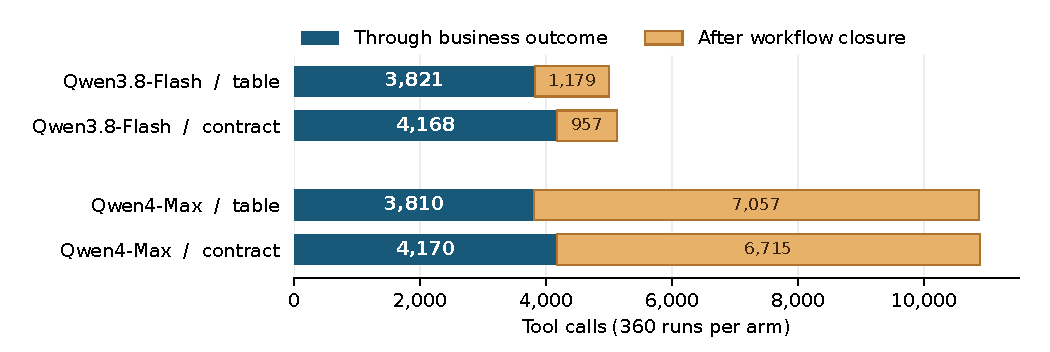
\includegraphics[width=\textwidth]{figures/strong-call-stages.pdf}
\caption{Tool calls through the business outcome and after workflow closure for the strong-baseline comparison. The shared original tool protocol remains in force for both models. The after-closure segment accounts for most of the Qwen4-Max aggregate cost.}
\label{fig:strong-stage-cost}
\end{figure*}

\subsection{Rule maintenance and audit}
We add three business rules covering changed bank details, cross-region pickup moves and restricted-site bookings. Both backends use three authored rule declarations. The table names three reusable recipe fragments. The contract configuration names four tools. The table additionally regenerates four existing and four new recipe entries. Both share the same generated business operation catalog. Both pass 36 policy fixtures, retain behavior on 12 old paths per backend, and detect all 15 injected faults per backend. Faults cover missing rules, selector changes, condition reversal, wrong field binding and missing prerequisites. The results measure configuration artifacts and regression coverage. Human authoring time and natural misconfiguration rates remain open.

Each backend emits enough information to reconstruct eight curated decisions after we add a shared structured log. It records rule identifiers, requested fields, prerequisites, and current and prepared evidence versions. Native contract logs include successful reads, while neither native interface carries the rule identifier in these cases. A separate reconciliation of approved rules and deployed configuration pinpoints all 15 faults per backend. The audit result therefore supports explicit instrumentation and configuration reconciliation for either implementation.

\subsection{Exploratory second-model compatibility}
A matched pilot runs six strong-baseline tasks with both backends using Qwen4-Max and compares the corresponding Qwen3.8-Flash records under the same tool protocol and budgets. Each model achieves 12/12 correct business outcomes and zero excess field releases. Qwen4-Max produces a normal final reply in 5/12 runs, compared with 12/12 for Qwen3.8-Flash. Tool calls rise from 158 to 340, with after-completion calls rising from 22 to 204. In this pilot the extra calls arise after the business outcome is settled. The strong-backend replication is reported in Section~\ref{sec:strong-autonomous}. Sections~\ref{sec:airgap-adaptation} and~\ref{sec:factorial} report the remaining replications. Token limits and finishing behavior are tracked separately from business completion.

In a separate matched diagnostic on six other tasks, we change only the response to a tool call after the workflow is closed. Both feedback formats achieve 12/12 correct business outcomes and zero excess releases. Explicit closure feedback increases normal final replies from 4/12 to 12/12 and cuts after-closure calls from 225 to 8. Calls before closure total 136 in each condition. This diagnostic isolates a tool-protocol effect on observed cost and is recorded separately from the full replication.

\subsection{Upfront minimization with escalation}
\label{sec:airgap-adaptation}
We evaluate a study-specific AirGapAgent-style adaptation with base-context minimization, a restricted conversational view and user escalation when additional fields are needed. The two on-demand arms begin with no private field values. The protocol uses 72 variants comprising 18 business-state pairs with both clean and externally injected tool text, two models, three arms and three repetitions (1,296 runs). This tests the adaptation on our workflows. The original AirGapAgent benchmarks and reported scores use different tasks and metrics.

\begin{table*}[t]
\centering
\small
\begin{tabular}{@{}llrrrrrr@{}}
\toprule
Model & Method & Correct & Unused & Data escalations & Action approvals & Tool calls & Model calls\\
\midrule
Qwen3.8-Flash & AirGap-style & 216/216 & 576 & 112 & 222 & 1927 & 2580\\
              & Agent only   & 216/216 & 0   & 0   & 222 & 1793 & 2011\\
              & State guard  & 216/216 & 0   & 0   & 222 & 1792 & 2012\\
Qwen4-Max     & AirGap-style & 216/216 & 366 & 182 & 222 & 2249 & 2896\\
              & Agent only   & 216/216 & 0   & 0   & 222 & 1900 & 2116\\
              & State guard  & 216/216 & 0   & 0   & 222 & 1963 & 2176\\
\bottomrule
\end{tabular}
\caption{AirGap-style adaptation and two on-demand controls. Unused fields are raw fields observed by the conversational agent that are outside the gold route field set. Data escalations ask for an additional field. Action approvals confirm the business operation.}
\label{tab:airgap-adaptation}
\end{table*}

Both on-demand arms eliminate observed unused fields in this study. The adaptation releases 576 and 366 unused field instances per model. With Qwen4-Max, the guard reduces tool calls by 286 and data escalations by 182 relative to the adaptation. All arms complete 216/216 tasks and preserve equal action approval counts. The exact-value checker finds no observed leakage and no unauthorized values delivered to the conversational agent. This comparison shows the effect of postponing disclosure under these policies. The separate stale-read settings in Sections~\ref{sec:autonomous} and~\ref{sec:strong-autonomous} test the need and cost of runtime enforcement.

\subsection{Query-order and enforcement ablation}
\label{sec:factorial}
A $2\times2$ study separates fixed versus planned predicate-query advice from advisory versus enforced reads. The contract and trusted predicates are shared. Each model uses three repetitions on 12 tasks per arm. We reproduce both archived versions of this study, one with native tool calls and one with JSON tool calls in model text, for 576 runs across models and interfaces. Table~\ref{tab:factorial} shows the Qwen4-Max replication.

\begin{table*}[t]
\centering
\small
\begin{tabular}{@{}lllrrrr@{}}
\toprule
Interface & Query advice & Read check & Correct & Stale fields & Predicate queries & Tool calls\\
\midrule
Native & Fixed   & Advisory & 36/36 & 12 & 12 & 292\\
       & Fixed   & Enforced & 36/36 & 0  & 12 & 294\\
       & Planned & Advisory & 36/36 & 12 & 9  & 288\\
       & Planned & Enforced & 36/36 & 0  & 9  & 291\\
Text   & Fixed   & Advisory & 36/36 & 12 & 12 & 344\\
       & Fixed   & Enforced & 36/36 & 0  & 12 & 348\\
       & Planned & Advisory & 36/36 & 12 & 9  & 345\\
       & Planned & Enforced & 36/36 & 0  & 10 & 340\\
\bottomrule
\end{tabular}
\caption{Qwen4-Max query-order and enforcement ablation. Stale fields are values delivered after the evidence supporting the read changed. Advice concerns the order of obtaining trusted predicates.}
\label{tab:factorial}
\end{table*}

Both models reproduce the twelve-to-zero stale-field contrast at each advice setting and in each interface. Qwen4-Max reaches 36/36 in every arm. With Qwen3.8-Flash, the same native arms achieve 36/36 and the archived text arms range from 33/36 to 34/36. Planned advice saves two to three predicate queries in the Qwen4-Max arms relative to fixed advice. Deployment conclusions about query cost remain bounded by the small predicate suite and its configured priors. The read check supplies the observed privacy effect in this ablation.

\subsection{Transfer to an independently maintained retail environment}
We use Sierra's retail environment from $\tau$-bench~\cite{taubench} as an external source of independently authored test annotations, synthetic order records, and executable business tools. We deterministically select 15 different target orders from 12 annotated test tasks. We preserve the annotated item and refund parameters for returns and the annotated cancellation inputs where available. The adapter calls the unmodified order lookup, address update, return, and cancellation functions. It projects the replies to the agent's view and uses fixed requests and simulated confirmations.

We construct state pairs for testing the delivery boundary. The same request initially authorizes updating the alternate address on a pending order. In the changed variant the simulator marks it delivered at a preassigned model turn. Some requests allow an annotated return; others require a safe stop. A third family first commits the cancellation of a separate order before the target order changes. The external benchmark supplies the retail tools and task material. The address-update branch, state schedule, conditional authorizations, and privacy scorer are part of our adaptation.

We compare agent-directed reads under the original task-level authorization, a composable refreshed route table, and the versioned contract backend. All arms share the same Qwen4-Max endpoint, prompts, tools, authority, confirmation and recovery policy. Thirty derived tasks and three repetitions per arm give 270 runs. We assess raw field releases against the currently valid route and score success from the upstream tool's actual simulated state changes and expected safe stops. The bounded cohort tests transfer of the enforcement mechanism to another tool implementation.

\begin{table*}[t]
\centering
\small
\begin{tabular}{@{}lrrrrrr@{}}
\toprule
Read policy & Correct & Excess fields & Block recovery & Calls through outcome & Calls after closure & Approvals\\
\midrule
Agent-directed & 90/90 & 270 & -- & 825 & 0 & 105\\
Refreshed route table & 90/90 & 0 & 45/45 & 780 & 0 & 105\\
Versioned contracts & 90/90 & 0 & 45/45 & 780 & 1 & 105\\
\bottomrule
\end{tabular}
\caption{Retail transfer study. Correct outcomes include 15 expected safe stops per arm. Block recovery is conditional on a denied field read. All arms produce 90 normal final replies.}
\label{tab:external-retail}
\end{table*}

The delivery event falls between read preparation and attempt in all 45 state-change runs per arm. Agent-directed reads deliver six obsolete address fields per changed run. Its confirmation check then sees that the address update is unavailable, so the agent still recovers. Both guarded arms stop the field release one tool call earlier. Each reduces observed excess fields from 270 to zero and saves 45 calls through the business outcome. The two guards match on correctness, excess exposure, and business-stage tool calls. All three arms deliver the prescribed safe stop on all 15 such runs. The result extends the observed delivery-time effect to independently developed retail tools, under our controlled state schedule. It does not estimate a passive rate of state changes or imply a score on the original benchmark protocol.

\subsection{Delivery-window and refund-rule maintenance studies}
\label{sec:refund-maintenance}
\paragraph{Is a decision at read preparation sufficient?}
We use three public Gaia2 Adaptability tasks~\cite{gaia2data} with upstream cancellation events and business scoring. After an initially valid catalog read starts, the experiment holds its reply until the original order cancellation. Qwen4-Max chooses all business actions. In seven same-task, same-seed triplets that reached the delivery window, agent-directed reads and a table refreshed at read preparation each delivered seven stale catalog replies. A contract checked at delivery returned zero stale replies and all three policies completed seven tasks. This is a controlled exposure opportunity on previously used public tasks. The outcome concerns the pending reply, including possible repeated delivery of an already observed identifier.

In a second run, the table also rechecked at delivery. Neither implementation delivered stale replies in the eight pairs that reached the window. The table completed eight and the contract six. Both generated the same value-free denial, and the two matched contract failures exhausted the response budget before the final user report. The paired post-switch tool totals were 59 and 58. These comparisons locate the benefit at the delivery boundary and leave production frequency unmeasured.

\paragraph{Which evidence should invalidate a pending read?}
We run Qwen4-Max on five synthetic refund trajectories with three seeds and three backends. A temporary wallet-priority change that returns to bank leaves bank authorization and the requested field versions intact. Binding all plan-support versions rejects three still-valid reads in this case. The narrower grant binds the bank authorization generation and the requested field versions, with current-route checking at delivery. It rejects all nine obsolete reads, reuses all six valid reads, and removes twelve downstream tool calls. The strengthened table, which also checks authorization generation and field versions, matches the narrow contract on all 15 pairs. All arms complete 15/15 refunds.

\begin{table}[t]
\centering
\small
\begin{tabular}{@{}lrr@{}}
\toprule
Metric & Table & Contract \\
\midrule
Workflow checks passed & 256/256 & 256/256 \\
Excess release cases & 0 & 0 \\
New authored declarations & 3 & 3 \\
Generated route recipes & 12 & 0 \\
Unchanged legacy checks & 32/32 & 32/32 \\
Structured decisions explained & 7/7 & 7/7 \\
Injected faults localized & 3/3 & 3/3 \\
\bottomrule
\end{tabular}
\caption{Refund rule changes under shared compilation and audit logging. Correct workflow checks include expected safe stops.}
\label{tab:refund-rule-maintenance}
\end{table}

\paragraph{What changes when business rules compose?}
We add three conditional checks to both the narrow contract and a composable table. Enhanced verification can serve both refund routes. A changed beneficiary adds a bank-only check. A large refund requires enhanced verification and review, and review waits for the beneficiary check when applicable. We freeze a factorial suite of four route states, eight trigger combinations, and eight field-authorization sets. A separate scripted ledger scores committed route, ordered prerequisites, released fields and approval. Table~\ref{tab:refund-rule-maintenance} summarizes the comparison. Both backends pass all 256 cases, committing 88 refunds and stopping safely in 168. The observed fields remain within the approved requirements in every case.

Both implementations use three authored overlay declarations with five route references and three dependency references. The shared compiler generates 31 action entries per backend from two original entries. It also materializes 12 table recipes from two original recipes, while the contract execution uses its action registry. The original authored entries remain intact. Bank-only, wallet-only and wallet-preferred flows require regression under the new rules. We also retain the no-route stop as a common check. With the new conditions disabled, all 32 legacy cases per arm preserve their prior outcomes and fields.

With a shared structured log, both implementations reconstruct all seven curated decisions, including valid composition, route change, authorization revocation, changed field version, an out-of-scope request, and a missing prerequisite. None of the five denied reads in either arm releases a raw value. Comparing approved declarations with deployed configuration locates each of three symmetric injected faults, and the corresponding regression supplies a counterexample. This study measures authored declarations, emitted artifacts and scripted diagnostic coverage. The shared compiler and log schema are setup costs, and developer time and naturally occurring mistakes remain open.


\section{Discussion}
\paragraph{What replicated.}
In the paired refund and logistics experiments, both hosted models release 144 stale field instances under agent-directed reads and zero with delivery-time checking. Business completion is 359/360 per policy for Qwen3.8-Flash and 360/360 for Qwen4-Max. Agent-driven recovery succeeds in 119 and 120 of the 120 blocked workflows, respectively. The core observation is temporal. A route can be eligible when the read is justified, then become ineligible before the values are returned. An execution-time check can preserve business correctness after the stale data has already reached the model.

The $\tau$-bench retail transfer reproduces the effect with independently developed order tools, order data, and test annotations. When a pending order is marked delivered, agent-directed reads still release the old address fields. Both guarded backends block these releases, reducing total excess field instances from 270 to zero. All three policies achieve 90/90 correct outcomes, including 15 expected safe stops per arm. Both guards recover in 45/45 blocked runs and save 45 tools through the business outcome by rejecting the read before the stale route reaches confirmation. This transfer crosses tool implementations on Qwen4-Max. The refund and logistics comparison separately tests replication across model aliases.

\paragraph{When the backends differ.}
The refreshed composable table recomputes field necessity for the current route and can accept a still-necessary read after a version change. The contract verifier also requires a previously prepared grant to match the versions of the evidence and fields it binds. This gives an explicit freshness guarantee for that grant. It can also force the agent to reprepare a read when refreshed business rules still permit delivery. Both implementations achieve zero excess releases in the direct comparisons. In Qwen4-Max's 90 version-only runs, binding adds 90 read denials and 360 tool calls through the business outcome. In the retail transfer, the two backends tie at 780 calls through the business outcome. Their recovery cost depends on whether changes invalidate the route or only the evidence version.

The narrowed refund contract ties a pending read to consent continuity and requested-field versions while refreshing route eligibility. It matches a table that enforces the same conditions. The rule-change experiment also finds equal authored maintenance, legacy regression scope, and structured audit coverage under shared tooling. The contract avoids emitting a separate set of route recipes in this implementation. Developer effort and naturally occurring misconfiguration rates remain unmeasured.

\paragraph{What independent authorship would test.}
The retail study uses upstream order tools, records and test annotations, with our state schedule and derived access policy. Gaia2 adds upstream tasks and cancellation events, with a delivery window that we control. A withheld study with independently authored tasks, event schedules and field requirements would test whether the findings generalize to other policies and continuations.

\paragraph{Scope and validity.}
The evidence comes from two hosted model aliases with unavailable exact serving snapshots and controlled sequential simulators. It leaves the prevalence of state changes and effects under concurrent production access open. The evaluation measures synthetic raw values entering model context and tests visible exact-value disclosure separately. Partial-value disclosure, semantic inference, hidden reasoning, compromised connectors, and unmediated reads are outside its measured scope. Tool overhead is reported separately through the business outcome and after workflow closure because the latter is sensitive to the model and the terminal reply format.

\section{Related work}
\paragraph{Contextual minimization.}
AirGapAgent first reduces a data view based on a trusted task context, isolates the conversational agent from the complete store, and can escalate a request to the user \cite{airgap}. Our setting targets the lifetime of a justified read after workflow execution has begun. An architectural adaptation in the artifact includes a minimizer, isolation and simulated escalation. Section~\ref{sec:airgap-adaptation} reports this study-specific adapter with its own metrics and protocol. The upfront arm of Table~\ref{tab:autonomous} is a release-policy comparator.

\paragraph{Tool policy and privacy measurement.}
CaMeL tracks provenance and allowed readers and enforces tool policies in an interpreter \cite{camel}. We study a different decision at the upstream delivery boundary: which fields a plan presently needs, given changes in supporting business evidence. Both controls could be composed. AgentDAM measures inappropriate private data use in autonomous web workflows \cite{agentdam}. \emph{Leaky Thoughts} studies exposure in visible reasoning and final outcomes, including the reconstructed AirGapAgent-R benchmark \cite{leaky}. These works motivate separate accounting for acquisition and downstream disclosure. Their benchmarks and reported rates are distinct from our synthetic business-workflow tasks.

\section{Conclusion}
Business-state changes can invalidate the reason for a read while task authorization stays fixed. Rechecking necessity immediately before raw delivery prevents overexposure under the tested changes. Value-free denial feedback lets the agent replan, continue from completed work, or stop safely. The reduction from agent-directed reading replicates across two hosted models and transfers to independently developed retail tools under our controlled state schedule. A composable route table with delivery-time checking matches the contract verifier on zero excess reads in the direct comparisons. Binding an authorization generation and the required field versions preserves grant freshness while allowing reuse after an irrelevant or temporary change. In the measured rule changes, both representations support composition and decision reconstruction under common tooling. The remaining evaluation will test this boundary on task pairs and state changes supplied independently of the mechanism design.

\section*{Ethics and artifacts}
Task profiles contain synthetic values. Confirmations and business operations are simulated. The artifact provides authored tasks, frozen protocols, traces, independent recounts, and plotting scripts. To preserve the anonymity of this review-format draft, repository URLs and author affiliations are omitted in the manuscript. The accompanying source package identifies the public experiment artifacts.

\bibliographystyle{plain}
\bibliography{references}
\appendix
\section{Autonomous protocol}
\label{sec:autonomous-protocol}
This appendix describes the design used in Section~\ref{sec:strong-autonomous}.

\paragraph{Question and arms.}
Compare reads, recovery and cost under two backends. Arm T composes route recipes and refreshes state at every read. Arm C derives requirements from tool contracts and validates an evidence-bound grant at delivery. Both share route eligibility, required fields, verification reuse, confirmation, idempotency and recovery rules.

\paragraph{Shared interface.}
Use one model snapshot, prompt, tool schema, response format, authorization policy, confirmation simulator and call budgets. A common prepare call returns an opaque handle: a request identifier in T and a grant identifier in C. Normalize denial codes and recovery advice for equivalent conditions. If a grant expires while its route remains viable, use common refresh-and-prepare guidance. The model issues all follow-up calls. Execution checks and scoring are shared.

\paragraph{Frozen paired tasks.}
The study uses 60 new pairs, 20 in each family below. Each pair shares the user request, synthetic values, starting authorization and tool capabilities. The two members vary a state update or its timing. Both arms run every member. Hold the 120 tasks out of prompt and policy development. Within the three families, include conditions where a supporting version changes but the current route remains admissible, to expose avoidable grant refreshes.
\begin{enumerate}
\item \textbf{Preferred route returns.} Change wallet availability before a pending raw read, with a matched case where the fallback stays necessary. The ledger checks the refund destination and whether any bank values were delivered.
\item \textbf{A committed action precedes replanning.} Change a booking prerequisite after a pickup-site change has committed. Vary whether a verification record is still valid for the new continuation. The ledger requires preservation of the committed effect and counts missing verification, redundant verification and duplicate commits.
\item \textbf{No authorized continuation.} Remove the active route when alternatives either lack authorization or cannot satisfy a business prerequisite. Pair it with a case retaining an authorized continuation. The ledger distinguishes an expected safe stop from an abandoned executable task. It records when a confirmation request is permitted.
\end{enumerate}

\paragraph{Timing and coverage.}
Freeze an event script per task. From a shared checkpoint (e.g., first status reply or committed pickup-site change), apply the update before tool dispatch at a predetermined later model turn. The schedule is independent of field requests, denials and grants. Preflight by replaying reference trajectories. Log checkpoint, event, preparation and delivery attempt separately. Report all runs and the share that reached the intended window by arm. Treat reached-window results as diagnostic because reaching it can depend on the arm.

\paragraph{Runs and scoring.}
Cross the 120 tasks with both arms and three repetitions for 720 runs. Counterbalance or randomize execution order within task and repetition. Use the same generation settings and matched seeds where the endpoint supports them. Start with the main study settings: a pinned version of \texttt{qwen3.8-flash}, temperature 0.3, up to 40 model responses, 512 output tokens per response and two recoveries. Log model version, calls and transport retries. Freeze the fixture ledger, model configuration and exclusions before running. Use scripted preflight to validate interface parity, environment resets and evaluator agreement. Keep refusals, timeouts and budget exhaustion in the assigned denominator, coded by failure cause.

An independent ledger scores the actual route, fields and business outcome against the rules at each event. Co-primary outcomes are excess raw fields (once per attempt, field and version) and correct outcomes, including expected safe stops. A field is excess if current shared business rules do not require it at delivery. Log grant expiration separately from business necessity. Separately report stale justifications, completion of executable tasks, recovery, repeated reads and verifications, duplicate effects, calls, confirmations and visible exact-value disclosure in text or outbound tools.

\paragraph{Analysis and interpretation.}
Report paired C-minus-T differences and 95\% bootstrap intervals resampling whole task pairs within family. Include per-family counts, discordances and failure traces. Freeze practical margins before any runs. Wide intervals leave parity unresolved. Similar privacy and completion under narrow intervals support the shared delivery rule on this suite. Maintenance claims require separate human effort and regression measurements.

\end{document}
